\providecommand{\main}{../../..}
\documentclass[\main/dresen_thesis.tex]{subfiles}
\renewcommand{\thisPath}{\main/chapters/theoreticalBackground/magnetism}
\begin{document}
\section{Magnetism}\label{ch:theoreticalBackground:magnetism}

  Classically, magnetic fields are understood to be produced by moving electric charges \cite{Jackson_1999_Class, Blundell_2001_Magne}.
  Within the framework of special relativity, magnetic fields emerge via a Lorentz transformation from the rest frame of an electric charge to a relatively moving one and the propagation and interaction of the magnetic field with charge and current distributions is fully described by Maxwell's equations.
  A central quantity to describe the sources of magnetic fields is the magnetic moment $\vec{\mu}$, which for localized current distribution $\vec{j}(\vec{r})$ is defined by
  \begin{align}
    \vec{\mu} \eq \frac{1}{2} \int \vec{r} \times \vec{j}(\vec{r}) \dint V .
  \end{align}
  In the case of a closed loop of current $I$, the magnetic moment is just given by the product of the current and the enclosed area $A$, $\mu \eq I A$, with the direction pointing parallel to the surface normal.
  The far-field generated by a magnetic moment is then given by the dipolar field
  \begin{align}
    \vec{B} (\vec{r}) \eq \frac{\mu_0}{4 \pi} \frac{3(\vec{\mu} \cdot \hat{r})\hat{r} - \vec{\mu}}{r^3}.
  \end{align}

  To understand the magnetism of matter, which is generally neutrally charged on the macroscopic scale, the motion of the electrons in the atoms needs to be evaluated\footnote{the direct contribution of the nucleus motion to the magnetism is approximately three orders of magnitude weaker due to the higher mass of the proton and neutrons relative to the electron}.
  The magnetic moment of an electron arises from the spin and orbital motion, which depends on the state the individual particle is in.
  Due to the quantum mechanical nature of the electron, the magnetic moment also needs to be treated quantum mechanically.
  In fact, the Bohr-van-Leeuwen theorem shows that for a purely classical system in thermal equilibrium, the magnetization is always zero.
  The various types of magnetism that are observed within different materials in nature can then be understood by the different structures and the effective couplings of the electrons, which in turn determines the direction of the many magnetic moments within the matter.
  The most popular types that are observed throughout this work are described in the following.

  \subsubsection{Diamagnetism}
    Diamagnetism is a weak effect that is exhibited by every material and measurable when it is not overshadowed by another type of magnetism.
    When a material enters a magnetic field, Faraday's law of induction states that currents are induced, which by Lenz's law are counter directed to the external field.
    For materials with $n$ electrons per volume, the diamagnetic magnetization can be described quantum mechanically in first order perturbation theory by the Langevin diamagnetism \cite{Blundell_2001_Magne}
    \begin{align}
      M \eq \underbrace{- \frac{n e^2}{6 m_e} \braket{r^2}}_{\eq \chi_D} B,
    \end{align}
    where $\braket{r^2}$ is the mean square distance of the electrons from the nucleus.
    The diamagnetic susceptibility $\chi_D$ is always negative and for common materials $\mu_0 \chi_D$ is in the order of $10^{-5}$.
    In magnetometry experiments, it is often observed from background materials such as a silicon substrate that carries the actual sample of interest or a solvent.
    As the Langevin diamagnetism is a linear function in $B$ that is largely temperature independent, it can in general be easily separated from other magnetic contributions if it is not negligible in strength.

  \subsubsection{Paramagnetism}
    Paramagnetism is observed in materials that have atomic or molecular orbitals with unpaired electrons.
    At zero field, if the magnetic moments are localized and decoupled, the direction of the moments is randomly distributed through thermal movement.
    Given an external magnetic field, the magnetic moments of the electrons feel a torque that tries to align the electron moment and field to minimize the Zeeman energy
    \begin{align}
      E_Z = - \vec{\mu}_e \cdot \vec{B}.
    \end{align}
    To determine the magnetization of a paramagnetic material at finite temperature and fields, Boltzmann statistics can be applied to obtain the partition function of the system and from this the magnetization.
    In a semiclassical approach, this leads to the formula for Langevin paramagnetism
    \begin{align}
      M \eq n \mu_e \Biggl( \coth \biggl(\frac{\mu_e B}{k T} \biggr) - \frac{k T}{\mu_e B} \Biggr).
    \end{align}
    For electrons, the energy scale of the Zeeman levels is $\mu_e B \ll kT$ and therefore
    \begin{align}
      M \approx \underbrace{\frac{n \mu_e^2}{3kT}}_{\eq \chi_P} B,
    \end{align}
    which shows that the paramagnetic susceptibility is positive and has a temperature dependance according to the Curie law $M \propto T^{-1}$.

  \subsubsection{Ferromagnetism, Antiferromagnetism, Ferrimagnetism}
    \begin{figure}[tb]
      \centering
      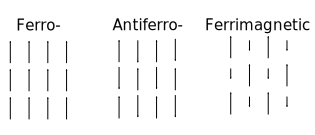
\includegraphics{magnetism_fm_afm}
      \caption{\label{fig:theoreticalBackground:magnetism:fm_afm_fim}Depiction of relative orientation and magnitude of the magnetic moments in a ferro-, antiferro- and ferrimagnetic material.}
    \end{figure}

    When a material has atoms with electrons in an unpaired state nearby to each other, it is generally possible that they couple for multiple reasons and thus affect the direction of their respective magnetic moments.
    A strong quantum mechanical effect between the spin of two electron emerges from the Coulomb interaction and the Pauli exclusion principle, which is known as the exchange interaction.
    Electrons with overlapping states can alter their charge distribution by aligning their spins $\vec{S}$ to one another and thus reduce their respective repulsion and the total energy of the system.
    This can effectively expressed by minimizing the exchange energy as given with the Heisenberg model
    \begin{align}
      E_{ex} \eq -\sum_{i \neq j} J_{ij} \vec{S}_i \cdot \vec{S}_j,
    \end{align}
    where $J_{ij}$ is the exchange integral that determines the coupling strength between two spins.
    Depending on the sign of $J_{ij}$, the energy is minimized by parallel alignment ($J_{ij} > 0$) or anti-parallel alignment ($J_{ij} < 0$).
    The parallel alignment is associated with a ferromagnetic state of the material, whereas the anti-parallel alignment is, depending on the relative magnitude of the magnetic moment in the two sub-lattices, is known as the antiferromagnetic or ferrimagnetic state as depicted in \reffig{fig:theoreticalBackground:magnetism:fm_afm_fim}.

    Even though the Heisenberg model captures the equal alignment between spins in a ferromagnet, it is isotropic and cannot describe anisotropies in a material.
    However, due to spin-orbit coupling and dipole-dipole interaction between the electrons, the shape and crystal structure of a material influences the magnetic behaviour and makes some direction in the crystal energetically favorable to another.
    Along this direction, called the easy axis, the magnetization of the material increases stronger than along another direction, whereas the saturation magnetization reached at high fields is independent of the direction.
    The anisotropy can be expressed phenomenology in dependence of the angle between the easy-axis and the direction of the magnetization and the crystal system.

    In this work, uniaxial and cubic anisotropies are considered.
    The uniaxial system is used to describe a single preferred direction as easy axis or when higher order terms in the anisotropy are negligible.
    If $\theta$ describes the angle between the easy-axis and the magnetization, the anisotropy energy is described by
    \begin{align}
      E_\mathsf{ani} \eq K_1 V \sin(\theta)^2,
    \end{align}
    with $K_1$ the material dependent anisotropy constant and $V$ the volume of the material.
    For cubic crystal systems, the anisotropy energy is given by
    \begin{align}
      E_\mathsf{ani} \eq
        \frac{K_1 V}{4} \biggl(\sin(2 \theta)^2 + \sin(\theta)^4 \sin(2\phi)^2 \biggr) +
        \frac{K_2 V}{16} \biggl( \sin(2 \theta)^2 \sin(2 \phi)^2 \sin(\theta)^2 \biggr),
    \end{align}
    where $\phi, \, \theta$ are the angle between the (001) direction and the magnetization direction in spherical coordinates.
    For $K_1 > 0$ and $K_2 > -9 K_1$ the \{100\} directions of the cubic system are the easy axis and for other values either \{110\} or \{111\} are the easy-axis.

    To minimize the magnetostatic energy necessary to maintain a large field outside of a ferromagnetic material, it becomes above a material dependent crystallite size energetically favorable to create separate domains of regions where the spins point into the same direction.
    The domain formation and the magnetic anisotropy both result in the characteristic hysteretic magnetization behaviour observed for ferromagnetic bulk materials below the order temperature.
    Ferromagnets show a hysteresis loop upon exposure to a sufficiently strong external magnetic field, with a remanent magnetization $M_R$ at removal of the field and the need of a coercive field $B_C$ to return the magnetization of the material to zero.

  \subsubsection{Superparamagnetism}
    When the crystallite size of a ferromagnetic material is reduced, domain formation is no longer energetically favorable below a material dependent critical size, which is typically in the order of nanometers.
    At this point, the crystallites are single domain and the spins of the individual electrons add to a single superspin.


  \subsection{Cobalt Ferrite and Maghemite}

\end{document}